\documentclass{article}

\usepackage{tikz}

\begin{document}
    \begin{center}
        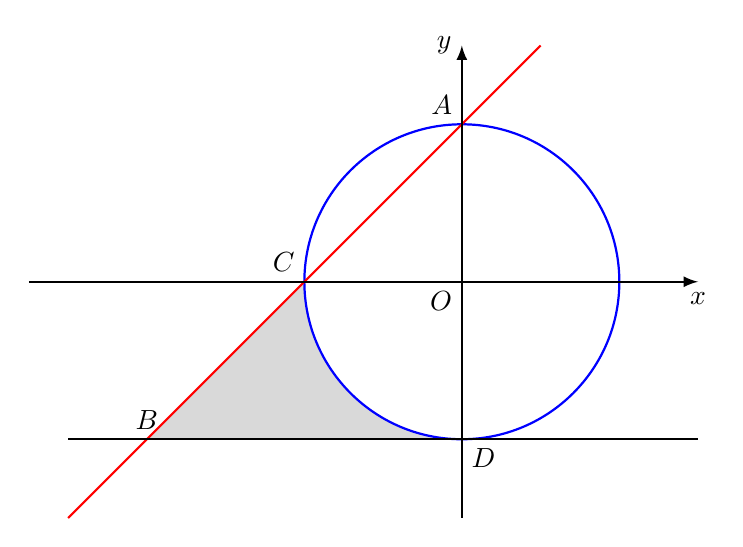
\begin{tikzpicture}
            \fill [gray!30] (-2,0) -- (-4,-2) -- (0,-2) -- cycle;
            \draw[thick, blue, fill=white] (0,0) circle (2cm);
            
            \draw[thick, red] (1,3) -- (-5,-3);
            \draw[thick] (-5,-2) -- (3,-2);
            \draw[thick,->, >=latex] (-5.5,0) -- (3,0) node[below] {\(x\)};
            \draw[thick,->, >=latex] (0,-3) -- (0,3) node[left] {\(y\)};
            
            \node at (0,0) [below left]{\(O\)};
            \node at (0,2) [above left]{\(A\)};
            \node at (-2,0) [above left]{\(C\)};
            \node at (-4,-2) [above]{\(B\)};
            \node at (0,-2) [below right]{\(D\)};
        \end{tikzpicture}
    \end{center}
\end{document}